\subsection{Broadcast: why local agreement need not improve reasoning}
\label{sec:broadcast}\label{sec:trajectory}

Under JustRL-1.5B, both DeepSeek-R1-Distill-Qwen-1.5B and Qwen2.5-1.5B-Instruct substantially reduce their training loss. Yet DeepSeek gains accuracy (\cref{sec:local}), while the base Qwen 1.5B model declines substantially on MATH within 100 steps. Why does learning from the same teacher help one learner and harm the other?

\paragraph{How do OPD updates change a per-prefix readout function?}
Let us first examine how an OPD update influences a local, per-prefix readout function of a rollout, such as the training loss or entropy. It acts on two coupled axes: it changes \emph{which prefixes} are encountered in future rollouts from the model, and it changes the model's \emph{predictions at a fixed prefix}. 

More precisely, let us define a local \emph{prefix readout} $Y_t(x)$. Define $J_Y(t)=\Ex_{\nu_t}Y_t(x)$, where $\nu_t$ is the observed prefix population. Then its rate of change (due to the parameter update) decomposes into ``routing'' and ``drift'':
\begin{equation}
 \dot J_Y(t)=
 \underbrace{\sum_x\dot\nu_t(x)Y_t(x)}_{R_Y(t):\ \text{routing}}
 +\underbrace{\Ex_{\nu_t}\dot Y_t(x)}_{D_Y(t):\ \text{drift}},
 \qquad J_Y(b)-J_Y(a)=\int_a^b(R_Y+D_Y)\,dt.
 \label{eq:rd-law}
\end{equation}
Drift changes the local, per-prefix readout over the current training population, while routing changes the probability weight assigned to the current prefixes, that is, which prefixes get exposed to teacher supervision in future updates.

At the more fundamental level of OPD's dynamics, both of these channels are projections of the $K$-$\Gamma$ broadcasts. The distinction is \emph{where the same update broadcasts}. Recall from the response law that the weighted request population $\Gamma_t$ propagate through $K_t$ to induce a logit response $v_t(x)$ at every receiver prefix $x$. With a temperature-$\tau$ sampler, receiver $x$ and prediction token $a$, this gives token log-probability velocity
\begin{equation}
 \zeta_t(x,a)=\partial_t\log\pi_t(a\mid x)
 =\frac{(e_a-\pi_t(\cdot\mid x))^\top v_t(x)}{\tau},
 \qquad v_t(x)=\sum_sK_t(x,s)\Gamma_t(s).
 \label{eq:rd-velocity}
\end{equation}
At the observed prefix $x$ itself, $v_t(x)$ changes its prediction, giving \emph{drift} $D_Y=\Ex_{\nu_t}[\nabla_zY_t(x)^\top v_t(x)]$. To reach that prefix, however, the autoregressive model must first generate its ancestor tokens, which also are the receivers of the $K$-$\Gamma$ broadcast. Summing the log-probability velocity of the ancestor tokens gives the velocity of reach-probability of prefix $x$, $\lambda_t(x)=\sum_{j<h(x)}\zeta_t(x_j,a_j)$. This gives \emph{routing} $R_Y=\operatorname{Cov}_{\nu_t}(Y_t,\lambda_t)$. 
Furthermore, the prefix visitation change causes the future training prefix distribution $\mu$ to change: within any time interval $[a,b]$,
\begin{equation}
 \mu_b(s)\propto\mu_a(s)e^{\Lambda_{a:b}(s)},\qquad
 \Lambda_{a:b}(s)=\int_a^b\lambda_t(s)\,dt\;\;\rightarrow \;\Gamma_b=\mu_bB_b.
 \label{eq:broadcast-source-renewal}
\end{equation}
The new rollouts (i.e. visited prefixes) supply the next requests and the induced $\Gamma$ field, on which the new round of updates and broadcasts are made. 

Intuitively, significant prefix-visitation change can be \emph{either} beneficial or damaging. For a weak student, it can route into low-quality, chaotic rollout distributions on which the teacher struggle to give requests that can help recover (or raise) the student's intermediate reasoning performance and terminal scores. On the flip side, the continually refreshed training rollouts also allow the possibility of ``online corrections'', where problematic reasoning behaviors broadcasted from early training can be corrected by the teacher mid-training. We will see these effects in our empirical analysis later.

To empirically study the effects of routing and drift in influencing the local readouts, we estimate their effects by \emph{cross-scoring training rollout banks and learners} at time intervals. Write $M_{ij}=\Ex_{x\sim\nu_i}Y_j(x)$ for the average readout of learner $j$ on the frozen bank of rollouts extracted at time step $i$, with $i,j\in\{a,b\}$. Replacing the bank at a fixed learner checkpoint measures routing; replacing the checkpoint on a fixed bank measures drift. Averaging the two replacement orders gives
\begin{equation}
 \widehat R_{a:b}=\tfrac12[(M_{ba}-M_{aa})+(M_{bb}-M_{ab})],\qquad
 \widehat D_{a:b}=\tfrac12[(M_{ab}-M_{aa})+(M_{bb}-M_{ba})].
 \label{eq:rd-estimators}
\end{equation}
These contributions sum exactly to $M_{bb}-M_{aa}$. Our curves accumulate them over consecutive windows; its relation to the path integrals and further details are in \cref{app:rd-theory,app:rd-protocol}\footnote{While a step-wise estimate for routing and drift is theoretically recommended, it is too expensive for our setting, and we resort to intervals of 20 update steps.}.

\paragraph{From local readouts to rollout-outcome readouts.}
So far we have discussed how the $K$-$\Gamma$ broadcasts change the model's predictions per prefix, how they accumulate along ancestor tokens to change prefix visitation, and how they influence a local per-prefix readout function. \emph{Correctness}, by contrast, is \emph{non-local}, and known only \emph{after completing the full rollout}, so its $J_Y$ expression must consider how ``aligned'' the policy motion is with terminal score when cumulated along a rollout trajectory. 

Generally, given a trajectory-determined terminal readout function $Y$, set $J_Y=\Ex_{\Pi_t}Y$ and use the student's continuation values
$Q_t^Y(x,a)=\Ex_t[Y\mid x,a]$ and $V_t^Y(x)=\Ex_{a\sim\pi_t}Q_t^Y(x,a)$.
We obtain:
\begin{equation}
 \begin{aligned}
 J_Y(T)-J_Y(t_\star)
 &=\int_{t_\star}^{T}\sum_xd_t(x)\Ex_{a\sim\pi_t}\!\left[\zeta_t(x,a)\underbrace{(Q_t^Y(x,a)-V_t^Y(x))}_{\text{continuation advantage}}\right]dt\\[-1pt]
 &=\frac1\tau\int_{t_\star}^{T}\sum_{x,s}d_t(x)
 [\pi_t\odot(Q_t^Y-V_t^Y)](x)^\top K_t(x,s)\Gamma_t(s)\,dt,
 \end{aligned}
 \label{eq:broadcast-continuations}
\end{equation}
where $d_t(x)$ is the probability of reaching $x$. This weights motion by what the \emph{student} can achieve. When the favored alternatives have similarly unsuccessful continuations, fitting their next-token distributions can yield little accuracy progress overall (see \cref{app:outcome-proof} for the proof).

\begin{figure}[!t]
\centering
\captionsetup[subfigure]{font=footnotesize,skip=2pt,justification=centering,singlelinecheck=false}
\begin{subfigure}[t]{.243636\linewidth}
\centering
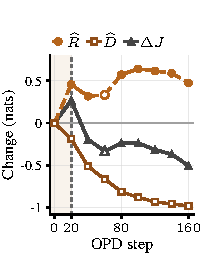
\includegraphics[width=\linewidth]{figures/section33/rd_loss_components.pdf}
\caption{Loss change}
\label{fig:rd-contrast-loss}
\end{subfigure}\hfill
\begin{subfigure}[t]{.243636\linewidth}
\centering
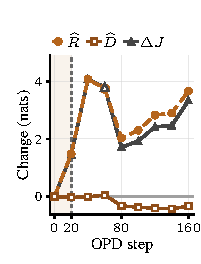
\includegraphics[width=\linewidth]{figures/section33/rd_entropy_components.pdf}
\caption{Entropy change}
\label{fig:rd-contrast-entropy}
\end{subfigure}\hfill
\begin{subfigure}[t]{.243636\linewidth}
\centering
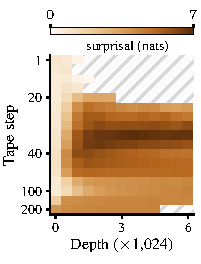
\includegraphics[width=\linewidth]{figures/section33/rd_student_uncertainty.pdf}
\caption{Student uncertainty}
\label{fig:rd-contrast-student}
\end{subfigure}\hfill
\begin{subfigure}[t]{.243636\linewidth}
\centering
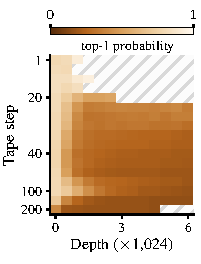
\includegraphics[width=\linewidth]{figures/section33/rd_teacher_confidence.pdf}
\caption{Teacher confidence}
\label{fig:rd-contrast-teacher}
\end{subfigure}
\caption{\textbf{Routing into unreliable prefixes, then fitting them.} Weak Qwen: (a,b) cumulative routing, drift, and total changes in local loss and entropy, each on its own scale. The vertical guide at step 20 marks the approximate onset-to-fitting transition; the effects overlap. (c,d) Student surprisal and teacher top-1 probability; darker means greater uncertainty. Columns are 512-token windows. Details are in \cref{app:rd-protocol}.}
\label{fig:rd-contrast}
\end{figure}

\paragraph{Weak 1.5B Qwen: routing into unreliable reasoning, then fitting uncertain supervision.}
In the early phase of training, the teacher pushes the weak learner toward longer rollouts (such as heavy negative requests on the student's ``overly early'' answer commitments), but these extensions become high-entropy and incoherent. The teacher supervision there also becomes much less concentrated than in the shallower rollout windows (\cref{fig:rd-contrast}c,d). As seen in \cref{fig:rd-contrast}(a) and (b), from step 1 to 20, loss rises $0.58\to0.85$ (routing $+0.455$ outweighs drift $-0.187$); entropy also rises mainly through routing. Intuitively, the student, which has never been trained to emit long reasoning rollouts, gets pushed into reasoning for long before committing an answer, and executing reasoning states which it is highly unfamiliar with. The teacher, conditioned on these low-quality states, also give much less confident guidance. 
The drift of the loss is small in this phase, however: the student has not learned the flatter prediction patterns of the teacher (uniformly) across the visited prefixes yet. 

What happens after the initial routing-dominated phase is dominated by drift (local fitting) on the unreliable request distributions. 
As seen in \cref{fig:rd-contrast}, entropy remains high within the band around $2-4$ nats, and loss reduction is increasingly driven by drift, that is, the student is indeed fitting the teacher's low confidence predictions on the chaotic, low-quality prefixes continually generated during training. To further test this, we find that, on the same batch-41 training prefixes, loss falls $0.79\to0.06$ while entropy falls $4.99\to3.99$: drift over the course of training actually broadcasts and sharpens predictions on this rollout bank toward an uncertain but slightly less entropic teacher (\cref{app:rd-entropy-response,app:rd-entropy-evidence}).

\paragraph{Policy motion and the shifting value of continuations.} So far we see that the weak Qwen model's failed run has the OPD update loop spending later, more ``stable'' drift-dominated updates learning from unreliable requests on the low-quality generative distribution. This helps us better understand how the training loss declines. Intuitively, fitting unreliable teacher supervision on high-entropy rollouts already suggests that this will not yield a better-reasoning student model. To understand how and why this process worsens terminal score more precisely, we need to turn to \Cref{eq:broadcast-continuations}: policy motion influences \emph{non-local} readouts (including terminal score) through the \emph{value / advantage} of the student's continuations (namely the $Q - V$ advantage summed across the prefixes), which can be in conflict with \emph{local} teacher agreement. 

While it is prohibitively expensive to directly compute the ``velocity$\times$advantage'' term in \cref{eq:broadcast-continuations}, we find on select banks of probing rollouts and continuations that as training proceeds, the model increasingly make local decisions whose continuation correctness decline, and complementarily, visit prefixes that are difficult to reach the right answer at increasingly shallower depth. This tells us that the per-token policy velocity of the model tend to align with ``negative advantage'' over the course of training, resulting in the overall decline of terminal accuracy. We elaborate on these studies below.

First, to probe the continuation-value term in \Cref{eq:broadcast-continuations}, we freeze a set of answer-decision prefixes from the initial student's held-out MATH rollouts and intervene on the local ``answer-versus-continue'' decision token position. The student's probability of the answer branch falls from $0.74\to0.19\to0.07$ at steps 0, 20, 100, below the teacher's $0.30$ on the same prefixes. At update 20, while ``routing'' is dominating, counterfactual continuations from the two branches have similar downstream value (correct $0.30$ for the ``answer'' branch and $0.29$ for the ``continue'' branch), i.e. the student still maintains reasonable answer-reaching abilities. By update 100, however, the continue-branch rarely produces the answer ($8\%$ of continuations). The teacher's own continuations from the same prefixes is correct $0.60$ of the time, which is much higher, so the gap is in the student's degraded execution of the action branch, not in the branch itself. For a complete treatment of how we decompose and estimate \cref{eq:broadcast-continuations} see \cref{app:steer-probe}. 


\begin{wrapfigure}{r}{.32\textwidth}
\vspace{-12pt}
\centering
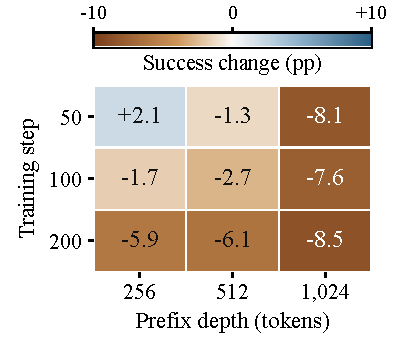
\includegraphics[width=\linewidth]{figures/section33/rd_initial_continuer.pdf}
\caption{\textbf{Initial-policy continuation success rate on trained prefixes.} Negative values indicate harder prefixes for reaching the right answer.}
\label{fig:rd-initial-continuation}
\vspace{-8pt}
\end{wrapfigure}

Now, these probes fix the prefixes and probe how the student checkpoints continues them. As we discussed before, the broadcast mechanism changes both prefix \emph{visitation} and continuations from them, therefore we next ask the complementary question of \emph{whether the prefixes visited during OPD also become increasingly harder to complete}. We fix a few rollout depths and student checkpoints, sample prefixes generated from these checkpoints at those depths, and then let the initial student (as a reference policy) to finish. Keeping the continuer \emph{fixed} makes changes in success reflect changes in prefix visitation. To understand the principled connections between these reference-continuer effects and \cref{eq:broadcast-continuations}, please refer to \cref{app:continuation-profile}. Empirically, \Cref{fig:rd-initial-continuation} shows a clear increase in continuation difficulty due to the prefix visitation shift, on the axes of rollout depths and training length. At step 50, while the shallow prefixes remains usable (even slightly better than the initial policy's own prefixes), it already yields less successful continuations on deep prefixes. As training goes on, the decline show up at increasingly shallower cuts of the rollout.


\begin{wrapfigure}{r}{.32\textwidth}
\vspace{-5.2em}
\centering
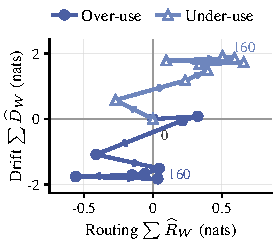
\includegraphics[width=\linewidth]{figures/section33/rd_deepseek_wait_side.pdf}
\caption{\textbf{Conditional checking refinement.} Filled circles: initial over-use; open triangles: initial under-use.}
\label{fig:rd-learning}
\vspace{-17pt}
\end{wrapfigure}


\paragraph{DeepSeek: stable learning acquiring epistemic behaviors.}



DeepSeek supplies the clean contrast. Loss falls $0.263\to0.015$, mainly through drift ($-0.214$) rather than routing ($-0.033$), indicating more more stable prefix visitations and local learning of requests. Furthermore, motivated by the epistemic-control request distribution found in \cref{sec:local}, we design a local readout to examine the dynamics of how the model acquires intermediate reasoning behaviors, focusing on ``wait''-family initiation at sentence starts (observed to initiate important backtracking and checking behaviors in R1-styled models \citep{marjanovic2026deepseekr}). On each prefix, let $w_t$ and $q_W$ denote student and teacher WAIT-family probabilities. We freeze two classes: \emph{over-use} ($w_0>q_W$) and \emph{under-use} ($w_0<q_W$), and set the local readout to be $\log[w_t/(1-w_t)]$ (log-odds of ``wait'' initiation).



\Cref{fig:rd-learning} plots cumulative routing and drift of the ``wait''-readout. Filled circles move downward: drift suppresses initial over-use. Open triangles move upward: drift promotes initial under-use. The corresponding net changes are $-1.82$ and $+1.92$ nats. While there are short overshoots of routing-dominated changes (early false suppression of under-use positions and promotion of over-use positions), they are quickly stabilized. Moreover, teacher-relative disagreement also decreases on frozen and held-out rollout banks (\cref{app:rd-checking}). Thus, unlike the failed learner's case where drift-dominated reduction of training loss happened on unreliable prefixes, DeepSeek's stabler drift-dominated reduction on training loss not only improves on its terminal score, but is accompanied by improvements in intermediate reasoning behaviors, with it sustaining prefix populations that allows to learn \emph{when} to initiate a ``wait''-based check as a representative example.


\paragraph{Preparation permits a different trajectory.}
The base Qwen model, prepared with offline distillation training on teacher rollouts, also undergoes substantial prefix visitation shifts, but sustains useful learning. Unlike DeepSeek's smoother refinement, its loss and checking behavior are nonmonotone: a routing-dominated overshoot in loss and reasoning (epistemic) behaviors are followed by lower-entropy rollouts and conditional moderation of reasoning behaviors dominated by drift. Its held-out gains suggest that a stronger starting policy with higher prefix quality and continuation-readiness makes these excursions amenable to correction. Full analysis in \cref{app:rd-prepared}.
